%% objective
Taking advantage of the modENCODE developmental data \citep{Graveley2011}, which contains expression data for 30 stages of the whole life cycle of \textit{D. melanogaster} (12 embryonic at 2-h intervals for 24 h, 6 larval, 6 pupal and 3 sexed adult stages at 1, 5 and 30 days after eclosion), $\omega_{\alpha}$ and other evolutionary rates for the genes expressed in each stage (for details see: IV, methods) were estimated.
For each stage, $\omega_{\alpha}$, $\omega$, $\omega_{d}$ and $\alpha$ (Fig. \ref{fig:Art-IV-OmegaA_lifecycle}) were estimated with the differentially expressed genes (genes with expression different from zero and excluding those expressed in all stages).

Also, different `genomic determinants' (codon usage bias, intron length, or number of exons) were estimated for each stage, in order to test how their temporal patterns would relate to the temporal patterns of the estimated evolutionary rates (i.e., $\omega_{\alpha}$, and others).




%% results OmegaA
The results show a clear temporal pattern, in which $\omega_{\alpha}$, $\omega_{d}$ and $\omega$ show their highest value at the first embryo stage (0-2hr) to then decrease until the 10-12hr embryo stage.
Their values remain low through most of embryonic development (the embryonic period were briefly discussed in section \ref{OmegaA_late_embryo}).
Then, from larval stage L3 the values increase suddenly and remain relatively high through all the pupa. 
Finally, in the adult stages, males show similar values to those of the pupa, but females show significantly lower values (p < 0.001). 

$\alpha$ follows a similar temporal profile to that of $\omega_{\alpha}$, but the differences in $\alpha$ values through the life cycle are smaller than those of $\omega_{\alpha}$.

Similar results were found when considering genes with a two-fold difference between maximal and minimal expression (IV, Fig S1), after excluding immune system and testes genes (IV, Fig. S2) or when the mutation rate is estimated using the 4-fold degenerate sites (IV, Fig. S3).

%%%%%%%%%%%%%%%%%%%%%%%%%%%%%%%%%%%%%%%%%%%%%%%%%%%%%%%
\begin{figure}[t]
  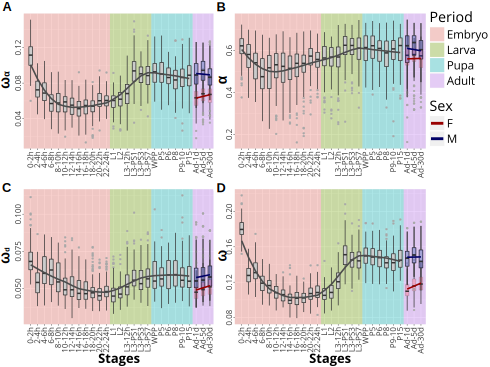
\includegraphics[width=0.9\textwidth]{./Images/Art-IV/OmegaA_lifecycle.png}
  \centering
  \caption{\textbf{ {\large$\omega_{\alpha}$} (A),  {\large$\alpha$} (B), {\large$\omega_{d}$} (C), {\large$\omega$} (D) through the life cycle of \textit{D. melanogaster}} Each time point represents 1,000 random samples of 350 genes (with replacement) expressed in a stage. Red line represents a LOESS regression. Female and male stages are fitted to a linear regression. There are 12 embryonic stages at 2hr intervals (from 0h to 24h). Larval stages at first instar (L1), second instar (L2) and third instar (L3). L3 stages are subdivided into the first 12 hours (L3-12h) and several puff stage (L3-PS1 to L3-PS7). WPP is the white pre-pupae stage. Pupal stages are phanerocephalic pupa, 15h (P5), 25.6 hours pupa (P6), yellow pharate, 50.4 hours (P8), amber eye-pharate, 74.6 hours (P9-10), green meconium pharate, 96 hours (P15). Adult stages are 1, 5 and 30 days after eclosion (Ad-1d, Ad-5d, Ad-30d).
  }
  \label{fig:Art-IV-OmegaA_lifecycle}
\end{figure}
%%%%%%%%%%%%%%%%%%%%%%%%%%%%%%%%%%%%%%%%%%%%%%%%%%%%%%%%

%% result genomic determinants

Most genomic determinants follow a temporal profile that is either very similar to that of $\omega_{\alpha}$ or the opposite of it (IV, Figs 2 and 3). 

Messenger complexity (number of transcripts divided by the number of exons) follows a very similar pattern to $\omega_{\alpha}$ (rank correlation $r^{2} = 0.622, p = 2.54x10^{-6}$ with the male stages and $r^{2} = 0.7, p =1.67x10^{-6}$ with female stages).
The temporal pattern of gene size, number of exons, codon usage bias and number of transcripts per gene patterns is the opposite of that $\omega_{\alpha}$  for males (rank correlations: $r^{2} = 0.702, p =1.66x10^{-6}$; $r^{2} = 0.867, p = 6.19x10^{-7}$; $r^{2} = 0.781, p = 1.27x10^{-6}$; $r^{2} = 0.667, p = 1.85x10^{-6}$, respectively) and females (rank correlations: $r^{2} = 0.697, p =1.68x10^{-6}$; $r^{2} = 0.888, p = 4.67x10^{-7}$; $r^{2} = 0.813, p =1.04x10^{-6}$; $r^{2} = 0.756, p =1.44x10^{-6}$, respectively). 

Using a fuzzy clustering algorithm, I found that genes that are expressed at high levels in the earliest development that rapidly decrease their expression to very low levels (cluster 1 and 2; IV, Fig. 4) are likely responsible for the high $\omega_{\alpha}$, $\omega_{d}$, $\omega$ and $alpha$ values in the first embryonic stages (IV, Fig. 4).
Also, I found that a subset of genes whose expression increases only in the last stages of embryonic development  (cluster 8; IV, Fig. 4) showed high$\omega_{\alpha}$ and $\omega$(permutation test, p = 0.008).

Cluster 1 and 8, which showed high $\omega_{\alpha}$ also showed significantly low gene size, number of exons and number of transcripts (permutation test, p < 0.001).





We find that all pupa and adult male stages exhibit the highest levels of adaptive change while mid and late embryonic stages show high conservation. 

